\documentclass{standalone}
\usepackage{tikz}
\usepackage{ctex,siunitx}
\setCJKmainfont{Noto Serif CJK SC}
\usepackage{tkz-euclide}
\usepackage{amsmath}
\usetikzlibrary{patterns, calc,3d}
\usetikzlibrary {decorations.pathmorphing,decorations.pathreplacing,decorations.shapes}
\begin{document}
\small
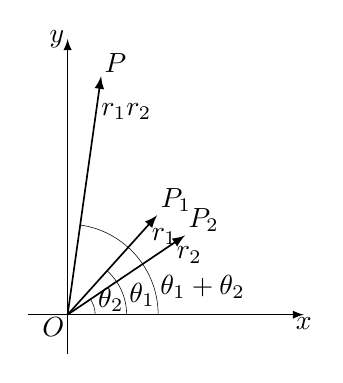
\begin{tikzpicture}[>=latex,scale=1.0,inner sep=1pt]
  \draw[->](-0.5,0)--(3,0)node[below]{$x$};
  \draw[->](0,-0.5)--(0,3.5)node[left]{$y$};
  \node at (0,0)[below left]{$O$};
  \draw[semithick,->](0,0)--(34:1.8)node[above right]{$P_2$}node[pos=0.9,below right]{$r_2$};
  \draw[semithick,->](0,0)--(48:1.7)node[above right]{$P_1$}node[pos=0.9,below right]{$r_1$};
  \draw[semithick,->](0,0)--(82:3.06)node[above right]{$P$}node[pos=0.9,below right]{$r_1r_2$};
  \draw[very thin](0.35,0)arc(0:34:0.35)node[at start,above right]{$\theta_2$};
  \draw[very thin](0.75,0)arc(0:48:0.75)node[pos=0.1,above right]{$\theta_1$};
  \draw[very thin](1.15,0)arc(0:82:1.15)node[pos=0.1,above right]{$\theta_1+\theta_2$};
\end{tikzpicture}
\end{document}